\chapter{Reti neurali (parte 1): dal neurone al MLP}\label{ch-06}

Con le reti neurali si entra nel cuore del corso. Questa prima parte
parte dall'ispirazione biologica, introduce il neurone artificiale e il
\textbf{Perceptron} con il suo algoritmo di apprendimento e il
\textbf{teorema di convergenza}, confronta il Perceptron con l'LMS,
introduce le funzioni di attivazione sigmoidali e arriva al
\textbf{Multi-Layer Perceptron} (MLP), analizzato come funzione
flessibile, come espansione in basi adattiva e come approssimatore
universale. Si chiude con i problemi che l'apprendimento in una rete
pone e che saranno risolti dalla \textbf{backpropagation}.

\section{Le reti neurali come strumento di
ML}\label{le-reti-neurali-come-strumento-di-ml}

Le reti neurali si studiano con due obiettivi diversi:

\begin{itemize}
\tightlist
\item
  \textbf{modellare sistemi biologici} e processi di apprendimento
  (filosofia, psicologia, neurobiologia, scienze cognitive, neuroscienze
  computazionali): qui il \textbf{realismo biologico} è essenziale;
\item
  \textbf{costruire sistemi e algoritmi di ML efficaci} (statistica, AI,
  fisica, matematica, ingegneria), spesso perdendo lo stretto realismo
  biologico: qui contano le proprietà \textbf{computazionali e
  algoritmiche}.
\end{itemize}

Nel corso ci interessano le \textbf{ANN} (\emph{Artificial Neural
Networks}) come \textbf{strumento flessibile di ML}, nel senso
dell'approssimazione di funzioni: una rete realizza una funzione
matematica \(h(\mathbf{x})\) con proprietà speciali.

Pur essendo una ``macchina storica'', le reti neurali restano un
approccio potente:

\begin{itemize}
\tightlist
\item
  apprendono da esempi;
\item
  sono \textbf{approssimatori universali} (teorema di Cybenko): approcci
  flessibili per funzioni arbitrarie, anche non lineari;
\item
  gestiscono rumore e dati incompleti, con prestazioni che
  \textbf{degradano gradualmente} in condizioni avverse;
\item
  trattano dati reali e discreti, per regressione e classificazione;
\item
  non sono un singolo modello ma un \textbf{paradigma} (nella classe
  degli approcci sub-simbolici).
\end{itemize}

La ``filosofia'' di fondo è il \textbf{connessionismo}: comportamenti
complessi (mentali, comportamentali) che \textbf{emergono}
dall'interazione di molte unità computazionali semplici interconnesse.

\section{L'ispirazione biologica}\label{lispirazione-biologica}

Il cervello umano ha più di \(10^{10}\) neuroni, ciascuno con
\(10^4\)--\(10^5\) connessioni. Un neurone risponde in circa un
millisecondo, eppure riconosciamo un'immagine in circa 0,1 secondi: al
massimo un centinaio di passi di calcolo \textbf{seriali}. Ne segue che
il cervello deve eseguire una computazione \textbf{massicciamente
parallela}. (Si noti che il riconoscimento facciale, così facile per
noi, è complesso per i computer convenzionali.)

\begin{figure}[htbp]
\centering
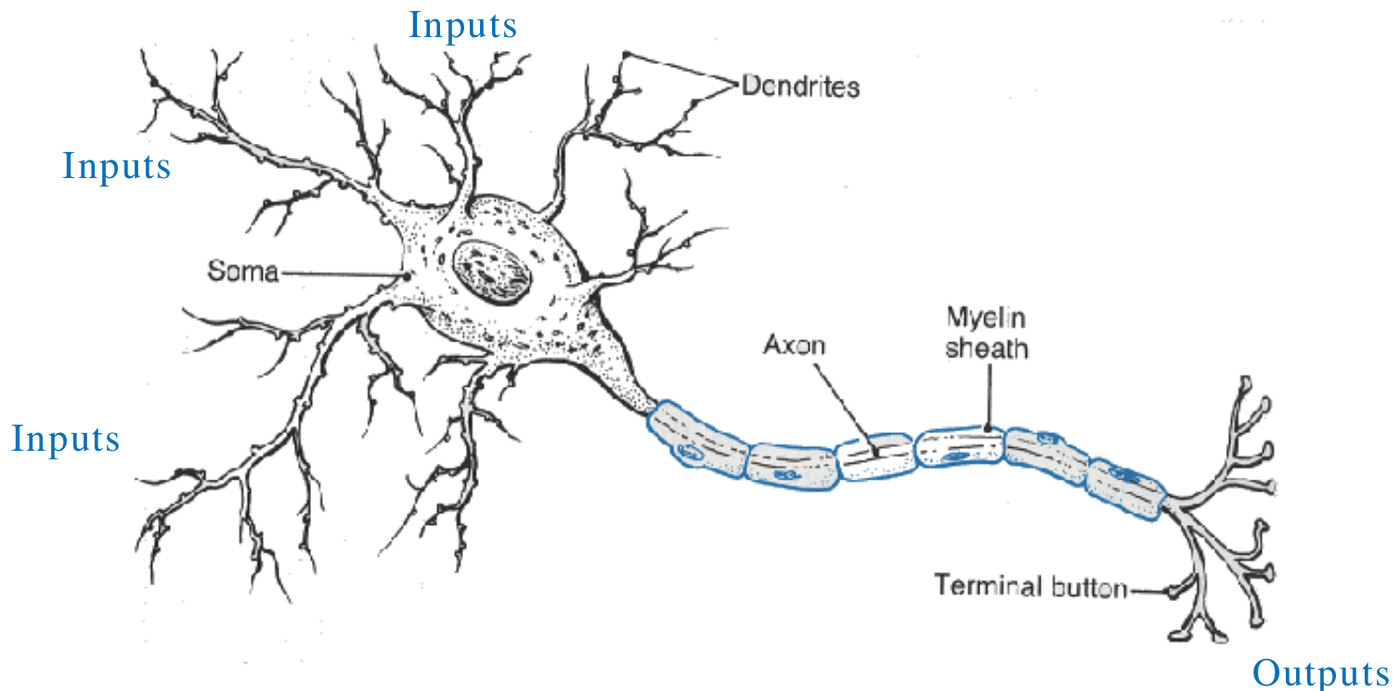
\includegraphics[width=0.80\linewidth,height=0.42\textheight,keepaspectratio]{images/06-nn1_neurone-biologico.png}
\caption{Il neurone biologico: dendriti (input), soma, assone e terminali
(output).}
\end{figure}

Il funzionamento, in sintesi: il neurone attraversa cicli di carica e
scarica (ioni sodio e potassio); gli input dai dendriti modificano il
potenziale della cellula; superata una \textbf{soglia}, viene generato
uno \textbf{spike} (un impulso di tensione), e l'informazione è
codificata anche negli intervalli di tempo tra gli spike.

Il segnale si propaga lungo l'assone fino alle \textbf{sinapsi}, dove
passa (in forma chimica, tramite \textbf{neurotrasmettitori}) al neurone
successivo. Le sinapsi possono essere \textbf{eccitatorie} o
\textbf{inibitorie}, e soprattutto cambiano con l'apprendimento: la loro
forza (il ``peso'') si rinforza in risposta agli stimoli. È la
\textbf{plasticità} del sistema nervoso.

\begin{boxdefinition}{Apprendimento hebbiano (Hebb, 1949)}

Una sinapsi si rafforza quando gli input del neurone (e gli output
correlati) si ripetono. Lo stimolo in ingresso rinforza la sinapsi,
quindi \textbf{i pesi si avvicinano agli input}.

\end{boxdefinition}

\section{Il neurone artificiale}\label{il-neurone-artificiale}

\begin{figure}[htbp]
\centering
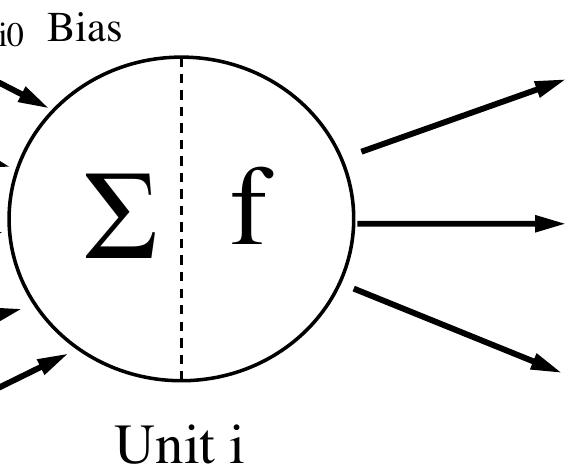
\includegraphics[width=0.43\linewidth,height=0.42\textheight,keepaspectratio]{images/06-nn1_unita.png}
\caption{L'unità di elaborazione (neurone artificiale).}
\end{figure}

Un'\textbf{unità} (nodo, neurone) riceve input da sorgenti esterne o da
altre unità. Ogni connessione ha un \textbf{peso} \(w\), parametro
libero modificabile dall'apprendimento (l'analogo della forza
sinaptica). L'unità \(i\) calcola: \[
net_i(\mathbf{x}) = \sum_j w_{ij}\, x_j, \qquad o_i(\mathbf{x}) = f\big(net_i(\mathbf{x})\big).
\]

\begin{itemize}
\tightlist
\item
  La somma pesata \(net_i\) è l'\textbf{input netto} (\emph{net input})
  dell'unità \(i\); include il bias \(w_{i0}\) tramite l'input costante
  \(x_0 = 1\).
\item
  \(f\) è la \textbf{funzione di attivazione} (lineare, a soglia,
  sigmoidale\ldots).
\end{itemize}

\begin{boxwarning}{Notazione dei pesi}

\(w_{ij}\) è il peso \textbf{dell'unità \(i\)}, cioè della connessione
\textbf{dall'input/unità \(j\) verso l'unità \(i\)} (non il contrario).
Alcune fonti (ad esempio Wikipedia nella sezione sulla backpropagation,
e alcune librerie) usano la convenzione opposta; nel corso si usa sempre
quella tradizionale: il primo indice è l'unità che riceve.

\end{boxwarning}

Tre funzioni di attivazione classiche:

\begin{figure}[htbp]
\centering
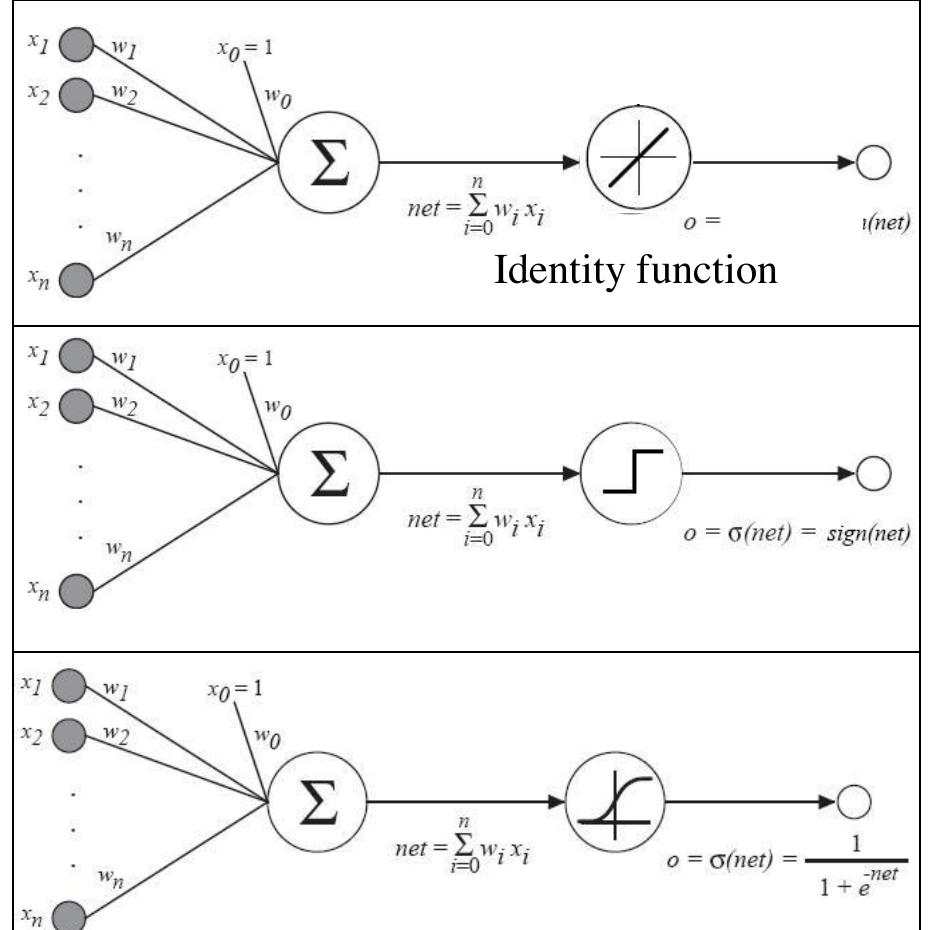
\includegraphics[width=0.54\linewidth,height=0.42\textheight,keepaspectratio]{images/06-nn1_attivazioni.png}
\caption{Funzione di attivazione lineare (identità), a soglia (Perceptron) e
logistica (sigmoide).}
\end{figure}

\begin{enumerate}
\def\labelenumi{\arabic{enumi}.}
\tightlist
\item
  \textbf{lineare} (identità): \(h(\mathbf{x}) = \sum_i w_i x_i\);
\item
  \textbf{a soglia} (gradino): è il \textbf{Perceptron}, cioè la LTU già
  vista;
\item
  \textbf{logistica} (sigmoide): vedi più avanti.
\end{enumerate}

\section{Il Perceptron}\label{il-perceptron}

Il \textbf{Perceptron} fu proposto da Frank Rosenblatt (1957--1960) per
la classificazione di pattern, simulando la percezione umana: un
``occhio'' di fotocellule collegato a unità che calcolano una
combinazione pesata con soglia.

\begin{figure}[htbp]
\centering
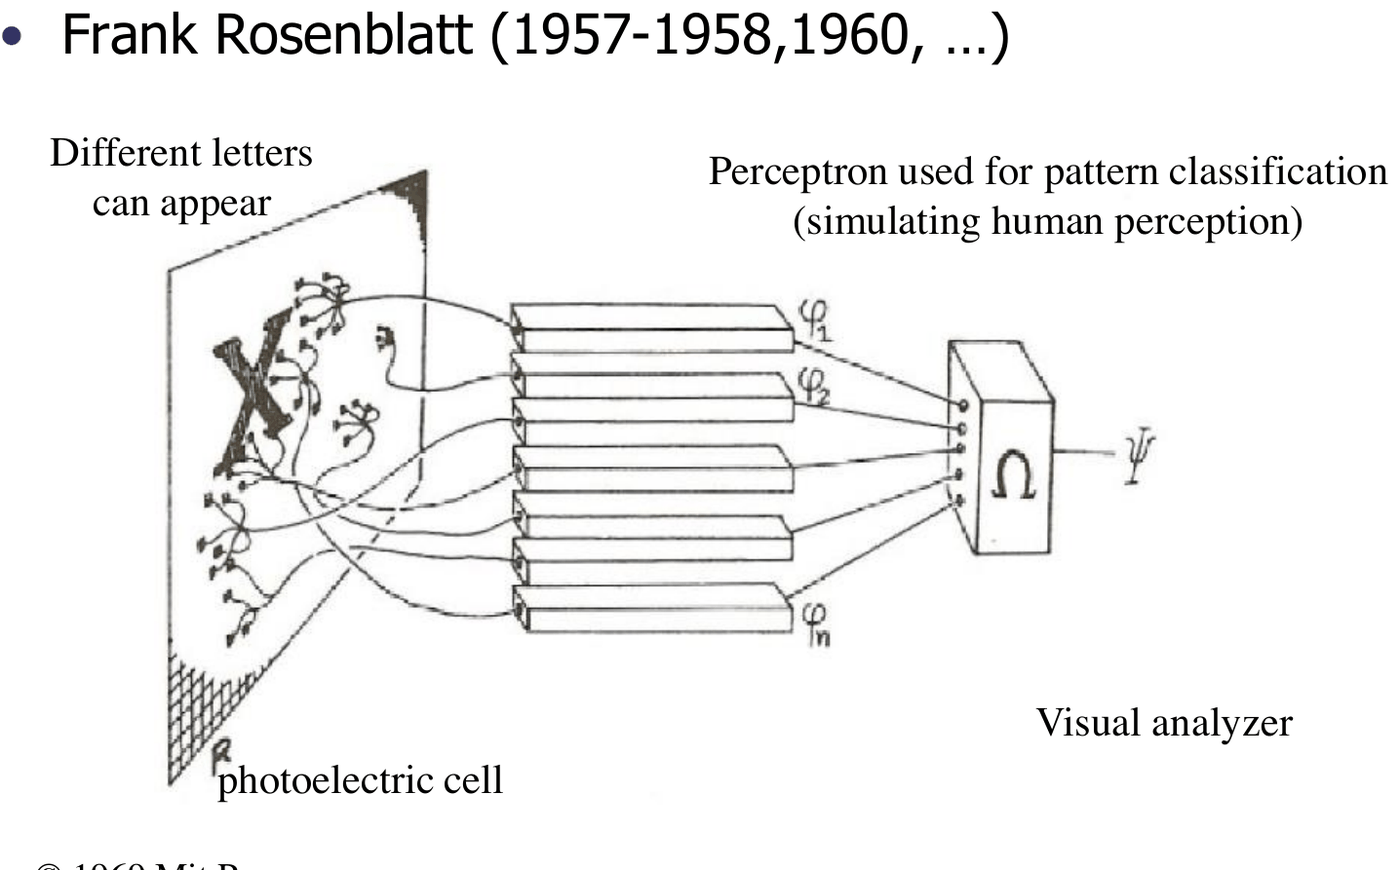
\includegraphics[width=0.63\linewidth,height=0.42\textheight,keepaspectratio]{images/06-nn1_perceptron-rosenblatt.png}
\caption{Il Perceptron originale, usato per riconoscere lettere.}
\end{figure}

Il singolo neurone è un'unità computazionale semplicissima. Minsky:
\emph{``per il tipo di riconoscimento che sa fare, è una macchina così
semplice che sarebbe sorprendente se la natura non la usasse da qualche
parte''}. Il Perceptron è un modello di importanza storica e
\textbf{paradigmatico} per il passaggio dai modelli lineari a quelli non
lineari: componendo e collegando perceptron si ottengono le reti
\textbf{MLP} (\emph{Multi-Layer Perceptron}).

\subsection{Le reti di McCulloch e Pitts
(1943)}\label{le-reti-di-mcculloch-e-pitts-1943}

Il primo modello, \emph{``A logical calculus of the ideas immanent in
nervous activity''} (1943), si chiedeva cosa calcola una rete data e se
una rete può calcolare una data formula logica.

\begin{itemize}
\tightlist
\item
  I neuroni hanno due stati: attivo (1) e non attivo (0).
\item
  Tutte le sinapsi sono equivalenti e caratterizzate da un numero reale
  (la forza \(w\)), positivo per connessioni \textbf{eccitatorie} e
  negativo per \textbf{inibitorie}.
\item
  Un neurone \(i\) si attiva quando la somma dei pesi \(w_{ij}\)
  provenienti dai neuroni \(j\) attivi, più un bias, supera zero.
\end{itemize}

Input e output binari: sostanzialmente è la LTU/Perceptron.

\subsubsection{Rappresentare funzioni
booleane}\label{rappresentare-funzioni-booleane}

Con \(net = \mathbf{w}^T\mathbf{x} = \sum_{i=0}^n w_i x_i\) e uscita
\(1\) se \(net > 0\), \(0\) (o \(-1\)) altrimenti:

\begin{itemize}
\tightlist
\item
  \textbf{AND}: \(w_1 = w_2 = 1\), \(w_0 = -1{,}5\) (serve che entrambi
  gli input valgano 1 per superare \(1{,}5\));
\item
  \textbf{OR}: \(w_1 = w_2 = 1\), \(w_0 = -0{,}5\) (basta un input a 1).
\end{itemize}

\begin{figure}[htbp]
\centering
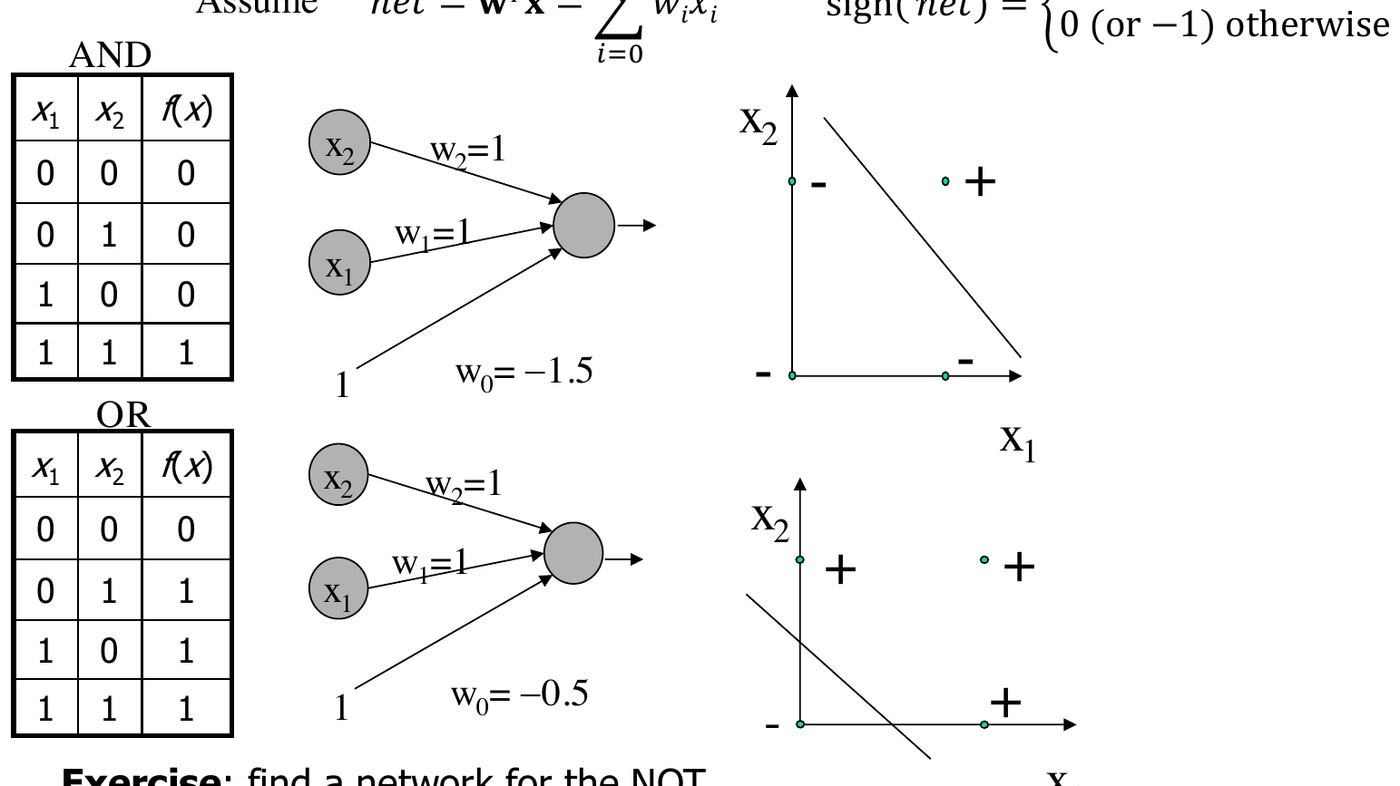
\includegraphics[width=0.80\linewidth,height=0.42\textheight,keepaspectratio]{images/06-nn1_and-or.png}
\caption{AND e OR realizzati da un singolo perceptron.}
\end{figure}

(Esercizio: il NOT si ottiene con \(w_1 = -1\), \(w_0 = 0{,}5\): per
\(x_1 = 0\) il net è \(0{,}5 > 0\), per \(x_1 = 1\) è \(-0{,}5\).)

\subsubsection{Lo XOR e le reti a due
strati}\label{lo-xor-e-le-reti-a-due-strati}

Lo \textbf{XOR} non è linearmente separabile: nessun singolo perceptron
lo può rappresentare (Minsky e Papert, 1969). Si può però scomporre: \[
x_1 \oplus x_2 = x_1\bar{x}_2 + \bar{x}_1 x_2 = \bar{h}_1 \cdot h_2, \qquad \text{con } h_1 = x_1 \cdot x_2 \text{ (AND)}, \quad h_2 = x_1 + x_2 \text{ (OR)}.
\]

\begin{boxtheorem}{XOR come composizione di AND e OR}

Per De Morgan,
\(\overline{h_1} = \overline{a \wedge b} = \bar a \vee \bar b\). Quindi
\[
\bar h_1 \wedge h_2 = (\bar a \vee \bar b) \wedge (a \vee b) = (\bar a \wedge a) \vee (\bar a \wedge b) \vee (a \wedge \bar b) \vee (b \wedge \bar b) = (\bar a \wedge b) \vee (a \wedge \bar b) = a \oplus b.
\]

\end{boxtheorem}

Si costruisce così una rete a \textbf{due strati}: due unità nascoste
calcolano \(h_1\) (AND) e \(h_2\) (OR), e un'unità di uscita calcola
\(\bar h_1 \wedge h_2\) (pesi \(-1\) da \(h_1\) e \(+1\) da \(h_2\),
bias \(-0{,}5\)).

\begin{figure}[htbp]
\centering
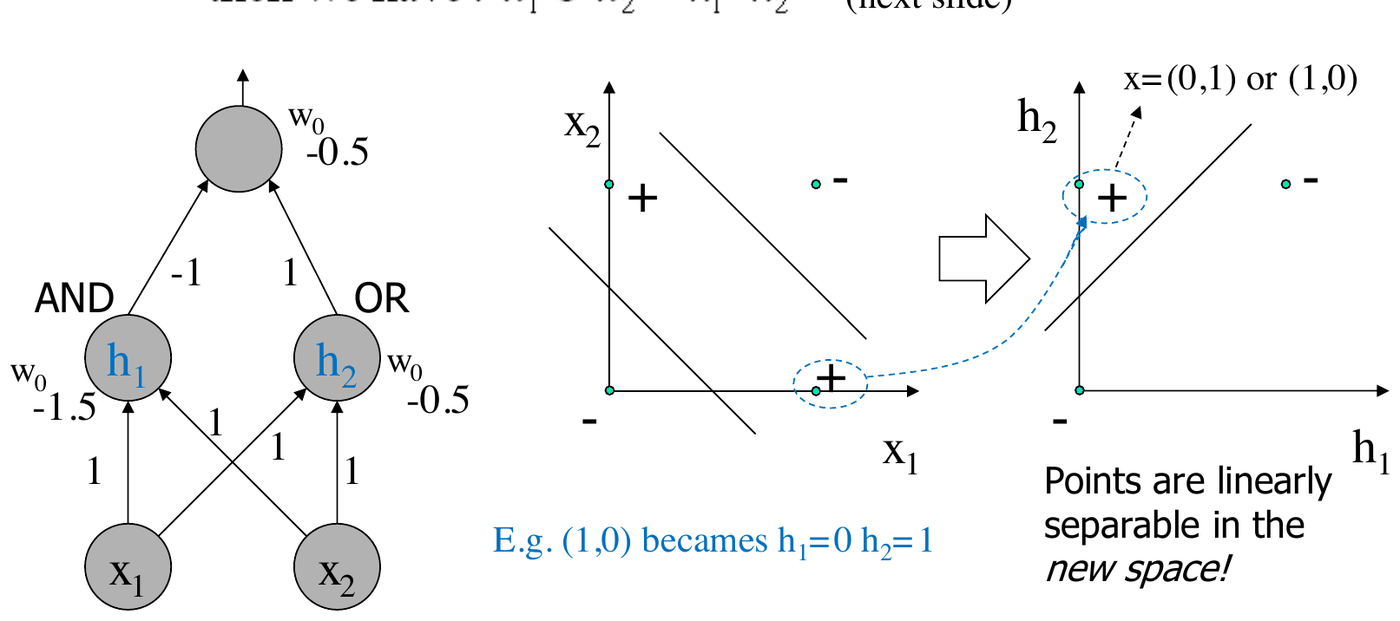
\includegraphics[width=0.89\linewidth,height=0.42\textheight,keepaspectratio]{images/06-nn1_xor-rete.png}
\caption{Lo XOR con una rete a due strati: nello spazio delle unità nascoste
\((h_1, h_2)\) i punti diventano linearmente separabili.}
\end{figure}

\subsection{Lo strato nascosto come
rappresentazione}\label{lo-strato-nascosto-come-rappresentazione}

La figura mostra il concetto chiave: lo strato nascosto produce una
\textbf{ri-rappresentazione interna} degli input. Il punto \((1,0)\),
che nello spazio originale sta nell'angolo in basso a destra, diventa
\(h_1 = 0\), \(h_2 = 1\): i due punti positivi \((0,1)\) e \((1,0)\)
vengono mappati \textbf{nello stesso punto} \((0,1)\) dello spazio
nascosto, e il problema diventa linearmente separabile per l'unità di
uscita.

\begin{boxtip}{Il concetto più importante delle reti neurali}

Sviluppare \textbf{feature di alto livello} negli strati nascosti è il
fattore chiave delle reti neurali: la rappresentazione nello strato
nascosto rende più facile il compito dello strato di uscita. Questa
composizione di operazioni intermedie può essere estesa su \textbf{molti
strati di astrazione}, e --- a differenza di quanto visto qui, dove i
pesi sono scelti a mano --- nelle reti neurali queste rappresentazioni
\textbf{si apprendono}. È l'idea alla base del \emph{representation
learning} e del \textbf{deep learning}.

\end{boxtip}

\begin{boxabstract}{Proprietà delle reti di perceptron}

\begin{itemize}
\tightlist
\item
  I perceptron rappresentano AND, OR, NOT (e quindi NAND, NOR) →
  \textbf{ogni funzione booleana} può essere rappresentata da una rete
  di perceptron.
\item
  \textbf{Due livelli} bastano (più livelli possono essere più
  efficienti).
\item
  Un singolo strato non basta (Minsky e Papert, 1969): limiti dovuti
  alla separabilità lineare.
\item
  Finora però \textbf{non abbiamo alcun algoritmo di apprendimento},
  nemmeno per una singola unità.
\end{itemize}

\end{boxabstract}

\section{Apprendimento per una singola
unità}\label{apprendimento-per-una-singola-unituxe0}

Storicamente ci sono due famiglie di metodi:

\begin{enumerate}
\def\labelenumi{\arabic{enumi}.}
\tightlist
\item
  \textbf{Adaline} (\emph{Adaptive Linear Neuron}, Widrow e Hoff):
  durante il training l'unità è \textbf{lineare}; si usano la soluzione
  diretta LMS o la discesa del gradiente (esattamente come nella lezione
  sui modelli lineari). Serve per regressione e, con la soglia,
  classificazione. È l'approccio che generalizzeremo agli MLP.
\item
  \textbf{Perceptron} (Rosenblatt): durante il training l'unità è
  \textbf{non lineare} (con funzione a soglia). Solo classificazione; se
  ne studiano le capacità e la convergenza.
\end{enumerate}

Per costruire un classificatore lineare abbiamo quindi tre algoritmi:
LMS diretto, LMS a gradiente e ora l'algoritmo del Perceptron (e altri
verranno, come le SVM).

\subsection{L'algoritmo di apprendimento del
Perceptron}\label{lalgoritmo-di-apprendimento-del-perceptron}

L'obiettivo è \textbf{minimizzare il numero di pattern classificati
male}: trovare \(\mathbf{w}\) tale che
\(\operatorname{sign}(\mathbf{w}^T\mathbf{x}) = d\). È un algoritmo
\textbf{on-line} (un passo per ogni pattern).

\begin{boxabstract}{Perceptron Learning Algorithm}

\begin{enumerate}
\def\labelenumi{\arabic{enumi}.}
\tightlist
\item
  Inizializzare i pesi (a zero o a piccoli valori casuali).
\item
  Scegliere un learning rate \(\eta \in (0, 1)\).
\item
  Finché non è soddisfatta la condizione di arresto (es. i pesi non
  cambiano più), per ogni pattern \((\mathbf{x}, d)\) con
  \(d \in \{+1, -1\}\):

  \begin{itemize}
  \tightlist
  \item
    calcolare \(out = \operatorname{sign}(\mathbf{w}^T\mathbf{x})\);
  \item
    se \(out = d\), \textbf{non cambiare i pesi};
  \item
    se \(out \ne d\), aggiornare:
    \(\mathbf{w}_{new} = \mathbf{w} + \eta\, d\, \mathbf{x}\).
  \end{itemize}
\end{enumerate}

\end{boxabstract}

In pratica si aggiunge \(\eta\mathbf{x}\) se
\(\mathbf{w}^T\mathbf{x} \le 0\) e \(d = +1\) (falso negativo), si
sottrae \(\eta\mathbf{x}\) se \(\mathbf{w}^T\mathbf{x} > 0\) e
\(d = -1\) (falso positivo). In forma equivalente: \[
\mathbf{w}_{new} = \mathbf{w} + \tfrac{1}{2}\eta\,(d - out)\,\mathbf{x},
\] perché \(d - out\) vale \(0\) se la classificazione è corretta e
\(\pm 2\) se è sbagliata.

\begin{boxwarning}{Differenza con LMS}

La formula sembra quella dell'LMS, ma qui \(out\) contiene il
\textbf{segno}: \(out = \operatorname{sign}(\mathbf{w}^T\mathbf{x})\),
mentre nell'LMS l'errore era calcolato su \(\mathbf{w}^T\mathbf{x}\)
(senza soglia).

\end{boxwarning}

\subsubsection{Vista geometrica}\label{vista-geometrica}

\begin{figure}[htbp]
\centering
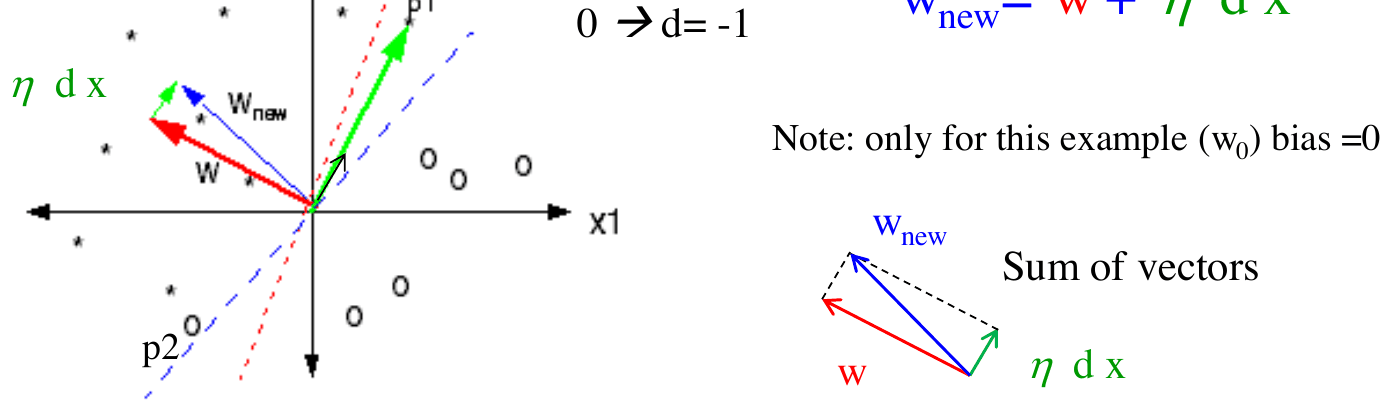
\includegraphics[width=0.86\linewidth,height=0.42\textheight,keepaspectratio]{images/06-nn1_perceptron-geometria.png}
\caption{Aggiornamento del Perceptron: \(\mathbf{w}\) viene spostato nella
direzione del pattern \(p_1\) mal classificato.}
\end{figure}

Prima dell'aggiornamento \(\mathbf{w}\) (che punta verso la regione
positiva) classifica male sia \(p_1\) sia \(p_2\). Scegliendo \(p_1\),
che ha target \(d = +1\), \(\mathbf{w}\) viene spostato di un po' nella
direzione di \(p_1\) (somma vettoriale
\(\mathbf{w} + \eta d\mathbf{x}\)), e il nuovo confine è migliore.
(Esercizio: se si sceglie \(p_2\), con \(d = -1\), \(\mathbf{w}\) viene
allontanato da \(p_2\).)

\subsection{Delta rule: due letture}\label{delta-rule-due-letture}

\begin{itemize}
\tightlist
\item
  La forma \(\mathbf{w}_{new} = \mathbf{w} + \eta\, d\,\mathbf{x}\) si
  può leggere come \textbf{apprendimento hebbiano}: \(\mathbf{w}\) si
  muove verso \(\mathbf{x}\).
\item
  La forma
  \(\mathbf{w}_{new} = \mathbf{w} + \eta\,(d - out)\,\mathbf{x} = \mathbf{w} + \eta\,\delta\,\mathbf{x}\)
  è una regola di \textbf{correzione dell'errore} (delta rule,
  Widrow-Hoff): il peso cambia in proporzione all'errore.
\end{itemize}

In termini di neuroni: \emph{la modifica di un peso sinaptico è
proporzionale al prodotto del segnale d'errore per il segnale di input
che eccita la sinapsi}. Il calcolo è facile quando il segnale d'errore
\(\delta\) è \textbf{direttamente misurabile}, cioè quando conosciamo la
risposta desiderata per l'unità. (Questo sarà il problema nelle reti con
strati nascosti.)

\subsection{Rappresentare e
apprendere}\label{rappresentare-e-apprendere}

Il Perceptron può \textbf{rappresentare} confini di decisione lineari,
quindi risolve i problemi linearmente separabili. Ma riesce sempre a
\textbf{imparare} la soluzione? Sì: il Perceptron con il suo algoritmo è
sempre in grado di apprendere ciò che può rappresentare.

\begin{boxnote}{Un risultato storico}

Il teorema di convergenza è una pietra miliare: un modello
\textbf{ispirato alla biologia}, con capacità computazionali ben
definite e \textbf{dimostrate matematicamente}.

\end{boxnote}

\subsection{Il teorema di convergenza del
Perceptron}\label{il-teorema-di-convergenza-del-perceptron}

\begin{boxtheorem}{Teorema di convergenza del Perceptron}

Se il problema è \textbf{linearmente separabile}, l'algoritmo del
Perceptron converge (classificando correttamente tutti i pattern) in un
\textbf{numero finito di passi}, indipendentemente dal punto di partenza
(anche se la soluzione finale non è unica e dipende dal punto di
partenza).

Se il problema non è separabile, l'algoritmo può essere instabile:
sviluppa \textbf{cicli}, con pesi non necessariamente ottimali.

\end{boxtheorem}

Nella dimostrazione omettiamo la \(T\) nei prodotti scalari tra vettori.

\subsubsection{Preliminari 1: ridursi a pattern tutti
positivi}\label{preliminari-1-ridursi-a-pattern-tutti-positivi}

Siano \((\mathbf{x}_i, d_i)\) gli esempi di training,
\(d_i \in \{+1, -1\}\), \(i = 1,\dots,l\). Se il problema è linearmente
separabile esiste una soluzione \(\mathbf{w}^*\) tale che \[
d_i(\mathbf{w}^*\mathbf{x}_i) \ge \alpha, \qquad \text{con } \alpha = \min_i d_i(\mathbf{w}^*\mathbf{x}_i) > 0.
\] Quindi \(\mathbf{w}^*(d_i\mathbf{x}_i) \ge \alpha\). Definendo
\(\mathbf{x}'_i = d_i\mathbf{x}_i\), \textbf{\(\mathbf{w}^*\) è una
soluzione del problema originale se e solo se è soluzione del problema
\((\mathbf{x}'_i, +1)\)} con tutti i target positivi:

\begin{itemize}
\tightlist
\item
  (se) \(\mathbf{w}^*\) risolve il problema originale
  \(\Rightarrow d_i(\mathbf{w}^*\mathbf{x}_i) \ge \alpha \Rightarrow \mathbf{w}^*\mathbf{x}'_i \ge \alpha \Rightarrow \mathbf{w}^*\)
  risolve \((\mathbf{x}'_i, +1)\);
\item
  (solo se) il ragionamento inverso.
\end{itemize}

Basta quindi dimostrare il teorema per un problema con \textbf{soli
pattern positivi}: ``ribaltare'' i pattern negativi non cambia nulla.

\subsubsection{\texorpdfstring{Preliminari 2: forma dei pesi dopo \(q\)
errori}{Preliminari 2: forma dei pesi dopo q errori}}\label{preliminari-2-forma-dei-pesi-dopo-q-errori}

Assumiamo \(\mathbf{w}(0) = \mathbf{0}\), \(\eta = 1\) e definiamo
\(\beta = \max_i \|\mathbf{x}_i\|^2\). Con soli pattern positivi, la
regola diventa \(\mathbf{w}(j) = \mathbf{w}(j-1) + \mathbf{x}_{i_j}\) a
ogni errore. Dopo \(q\) errori (tutti falsi negativi): \[
\mathbf{w}(q) = \sum_{j=1}^{q} \mathbf{x}_{i_j},
\] dove \(i_j\) indica i pattern classificati male (ad esempio gli
indici 2, 8, 9, 14 del training set; lo stesso pattern può comparire più
volte).

\subsubsection{Idea della dimostrazione}\label{idea-della-dimostrazione}

Si trovano un \textbf{limite inferiore} a \(\|\mathbf{w}(q)\|^2\) che
cresce come \(q^2\) e un \textbf{limite superiore} che cresce come
\(q\). Poiché una funzione quadratica supera prima o poi una lineare, i
due limiti sono compatibili solo per \(q\) fino a un certo valore
massimo: il numero di errori (e quindi di aggiornamenti) è finito.

\begin{figure}[htbp]
\centering
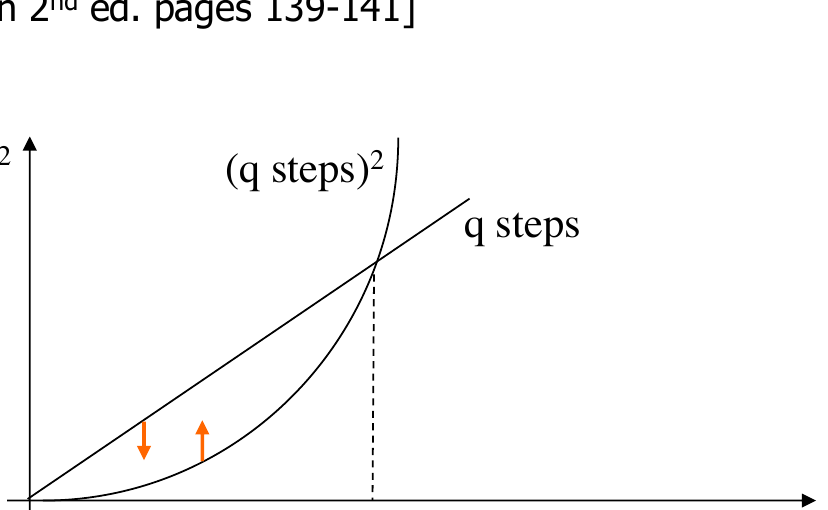
\includegraphics[width=0.54\linewidth,height=0.42\textheight,keepaspectratio]{images/06-nn1_convergenza.png}
\caption{Idea della dimostrazione: il limite inferiore quadratico e il limite
superiore lineare si incontrano in \(q_{max}\).}
\end{figure}

\subsubsection{Limite inferiore}\label{limite-inferiore}

\[
\mathbf{w}^{*T}\mathbf{w}(q) = \mathbf{w}^{*T}\sum_{j=1}^{q}\mathbf{x}_{i_j} \ge q\alpha,
\] perché ogni termine \(\mathbf{w}^{*T}\mathbf{x}_{i_j}\) è almeno
\(\alpha\). Per la \textbf{disuguaglianza di Cauchy-Schwarz},
\(\|\mathbf{a}\|^2\|\mathbf{b}\|^2 \ge (\mathbf{a}^T\mathbf{b})^2\); con
\(\mathbf{a} = \mathbf{w}^*\) e \(\mathbf{b} = \mathbf{w}(q)\): \[
\|\mathbf{w}^*\|^2\,\|\mathbf{w}(q)\|^2 \ge \big(\mathbf{w}^{*T}\mathbf{w}(q)\big)^2 \ge (q\alpha)^2 \quad\Rightarrow\quad \|\mathbf{w}(q)\|^2 \ge \frac{(q\alpha)^2}{\|\mathbf{w}^*\|^2}.
\]

\subsubsection{Limite superiore}\label{limite-superiore}

Usando
\(\|\mathbf{a} + \mathbf{b}\|^2 = \|\mathbf{a}\|^2 + 2\mathbf{a}\mathbf{b} + \|\mathbf{b}\|^2\):
\[
\|\mathbf{w}(q)\|^2 = \|\mathbf{w}(q-1) + \mathbf{x}_{i_q}\|^2 = \|\mathbf{w}(q-1)\|^2 + 2\,\mathbf{w}(q-1)\,\mathbf{x}_{i_q} + \|\mathbf{x}_{i_q}\|^2.
\] Poiché \(\mathbf{x}_{i_q}\) è stato classificato male (è il
\(q\)-esimo errore), \(\mathbf{w}(q-1)\,\mathbf{x}_{i_q} \le 0\):
eliminando questo termine non positivo si ottiene \[
\|\mathbf{w}(q)\|^2 \le \|\mathbf{w}(q-1)\|^2 + \|\mathbf{x}_{i_q}\|^2,
\] e iterando (con \(\mathbf{w}(0) = \mathbf{0}\)): \[
\|\mathbf{w}(q)\|^2 \le \sum_{j=1}^{q}\|\mathbf{x}_{i_j}\|^2 \le q\beta.
\]

\subsubsection{Conclusione}\label{conclusione}

Mettendo insieme i due limiti: \[
q\beta \;\ge\; \|\mathbf{w}(q)\|^2 \;\ge\; \frac{(q\alpha)^2}{\|\mathbf{w}^*\|^2} \quad\Rightarrow\quad q \le \frac{\beta\,\|\mathbf{w}^*\|^2}{\alpha^2}.
\] Il numero di errori (e quindi di aggiornamenti) è limitato da una
costante: l'algoritmo converge in un \textbf{numero finito di passi}.
\(\blacksquare\)

\begin{boxtip}{Interpretazione del bound}

Il numero di passi cresce con \(\beta\) (quanto sono ``grandi'' i
pattern) e decresce con \(\alpha^2\): \(\alpha\) misura quanto il
problema è ``ben separato'' (il margine minimo della soluzione
\(\mathbf{w}^*\)). Problemi con classi vicine all'iperpiano separatore
richiedono più passi. L'idea di \textbf{margine} tornerà centrale nelle
SVM.

\end{boxtip}

\section{Perceptron contro LMS}\label{perceptron-contro-lms}

Le due regole sembrano simili
(\(\mathbf{w}_{new} = \mathbf{w} + \eta\,\delta\,\mathbf{x}\)), ma:

\begin{itemize}
\tightlist
\item
  l'LMS è derivato (tramite il gradiente) \textbf{senza} funzione a
  soglia, minimizzando l'errore dell'unità lineare:
  \(\delta = d - \mathbf{w}^T\mathbf{x}\);
\item
  il Perceptron usa l'uscita con soglia:
  \(\delta = d - \operatorname{sign}(\mathbf{w}^T\mathbf{x})\).
\end{itemize}

Naturalmente il modello addestrato con LMS si può usare per classificare
applicando la soglia
(\(h(\mathbf{x}) = \operatorname{sign}(\mathbf{w}^T\mathbf{x})\), LTU).

Una conseguenza importante: \textbf{l'LMS può classificare male anche
problemi linearmente separabili}. L'LMS non minimizza il numero di
errori della LTU, ma l'errore quadratico, e modifica i pesi
\textbf{anche per i pattern già classificati correttamente}. Un pattern
corretto ma ``lontano'' dall'iperpiano (con \(\mathbf{w}^T\mathbf{x}\)
molto maggiore di 1) produce comunque un errore quadratico grande che
``tira'' l'iperpiano.

\begin{figure}[htbp]
\centering
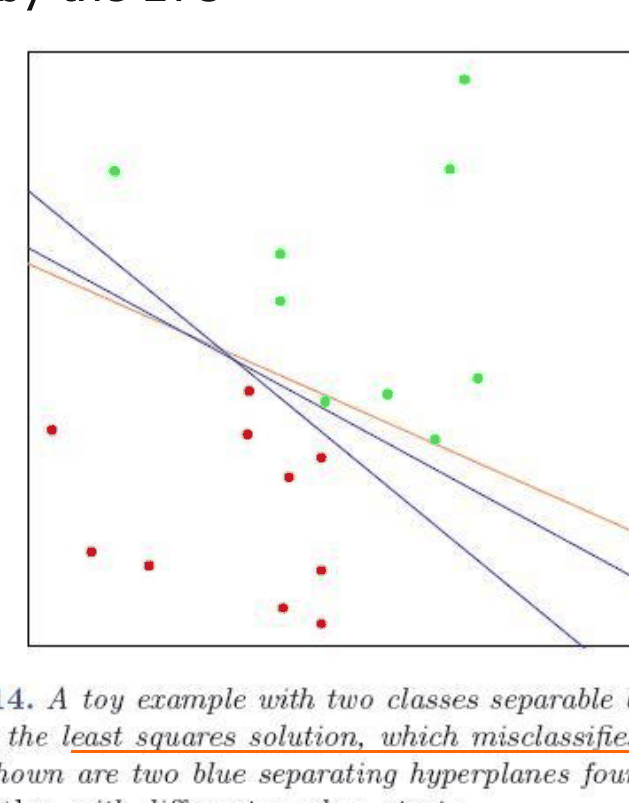
\includegraphics[width=0.43\linewidth,height=0.42\textheight,keepaspectratio]{images/06-nn1_lms-vs-perc.png}
\caption{Un problema separabile: la soluzione LMS (arancione) sbaglia un punto,
il Perceptron (blu, due diverse inizializzazioni) separa tutto (Hastie
et al., Fig. 4.14).}
\end{figure}

{\def\LTcaptype{none} % do not increment counter
\begin{longtable}[]{@{}
  >{\raggedright\arraybackslash}p{(\linewidth - 2\tabcolsep) * \real{0.5000}}
  >{\raggedright\arraybackslash}p{(\linewidth - 2\tabcolsep) * \real{0.5000}}@{}}
\toprule\noalign{}
\begin{minipage}[b]{\linewidth}\raggedright
Perceptron Learning Algorithm
\end{minipage} & \begin{minipage}[b]{\linewidth}\raggedright
LMS
\end{minipage} \\
\midrule\noalign{}
\endhead
\bottomrule\noalign{}
\endlastfoot
Minimizza le classificazioni errate
(\(out = \operatorname{sign}(\mathbf{w}^T\mathbf{x})\)) & Minimizza
\(E(\mathbf{w})\) con \(out = \mathbf{w}^T\mathbf{x}\) \\
Converge sempre per problemi separabili, in un numero finito di passi, a
un classificatore perfetto & Convergenza \textbf{asintotica}, anche per
problemi non separabili \\
Non converge se il problema non è separabile & Non sempre zero errori di
classificazione, anche su problemi separabili \\
Difficile da estendere a reti di unità & \textbf{Estendibile a reti} con
l'approccio a gradiente \\
\end{longtable}
}

L'ultima riga è decisiva: per costruire reti neurali serve un approccio
basato sul \textbf{gradiente}, che richiede funzioni differenziabili.

\section{Funzioni di attivazione
sigmoidali}\label{funzioni-di-attivazione-sigmoidali}

Oltre alla lineare e alla soglia, si usano funzioni \textbf{non lineari
``a schiacciamento''} (\emph{squashing}) come la \textbf{sigmoide
logistica}, che assume valori continui nell'intervallo limitato
\([0,1]\): \[
f_\sigma(x) = \frac{1}{1 + e^{-ax}}.
\] È una \textbf{versione liscia e differenziabile della funzione
soglia}. Il parametro \(a\) è la \textbf{pendenza} (\emph{slope}).

\begin{figure}[htbp]
\centering
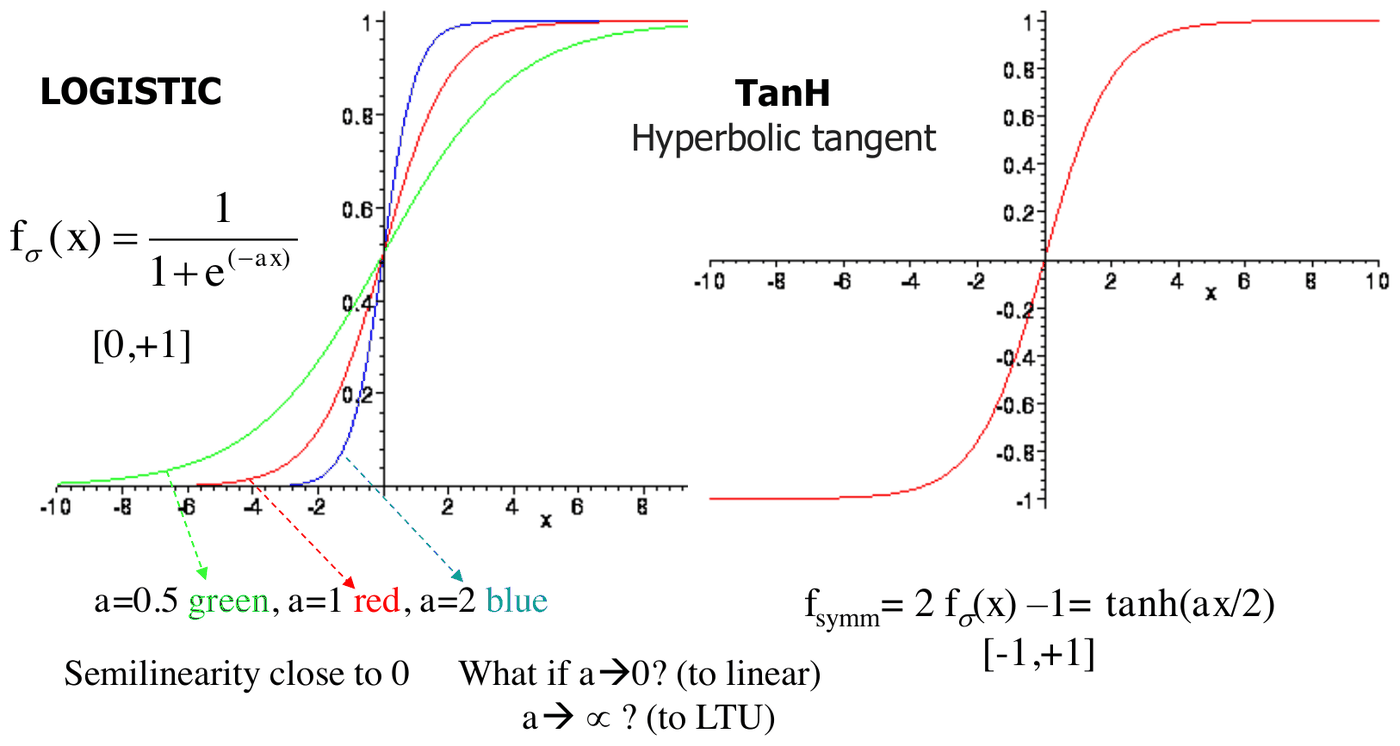
\includegraphics[width=0.91\linewidth,height=0.42\textheight,keepaspectratio]{images/06-nn1_sigmoidi.png}
\caption{Sigmoide logistica (sinistra) per diversi valori di \(a\) e tangente
iperbolica (destra).}
\end{figure}

La versione simmetrica è la \textbf{tangente iperbolica}, con valori in
\([-1, +1]\): \[
f_{symm}(x) = 2f_\sigma(x) - 1 = \tanh(ax/2).
\]

Vicino a zero la sigmoide è quasi lineare (\textbf{semi-linearità}). Al
variare di \(a\):

\begin{itemize}
\tightlist
\item
  per \(a \to 0\) la funzione tende a una funzione \textbf{lineare}
  (molto piatta);
\item
  per \(a \to \infty\) tende alla funzione \textbf{a gradino} (LTU).
\end{itemize}

Per la classificazione, con la logistica un'uscita \(\ge 0{,}5\)
corrisponde alla classe positiva e \(< 0{,}5\) alla classe zero/negativa
(per la tanh la soglia è 0). La soglia si può spostare (studiando
l'effetto su falsi positivi/negativi o con una curva ROC), e si può
anche definire una \textbf{zona di rifiuto} attorno alla soglia per
evitare decisioni fragili.

\subsection{Altre funzioni di
attivazione}\label{altre-funzioni-di-attivazione}

\begin{itemize}
\tightlist
\item
  \textbf{Funzioni a base radiale} (RBF): \(f(x) = e^{-ax^2}\) applicata
  a \(\|\mathbf{w} - \mathbf{x}_{input}\|\), cioè una gaussiana centrata
  sui pesi → \textbf{reti RBF}.
\item
  \textbf{Softmax}: per il caso con uscite multiple (vedi lezioni
  successive).
\item
  \textbf{Neuroni stocastici}: uscita \(+1\) con probabilità \(P(net)\),
  \(-1\) altrimenti → \textbf{macchine di Boltzmann} e modelli della
  meccanica statistica.
\item
  Approssimazioni \textbf{lineari a tratti} della tanh, per calcoli
  efficienti (anche con shift binari).
\item
  \textbf{ReLU} (\emph{Rectified Linear Unit}): \(f(x) = \max(0, x)\). È
  diventata la scelta predefinita per i modelli profondi; se ne parlerà
  nel deep learning.
\item
  \textbf{Softplus}, la sua approssimazione liscia:
  \(f(x) = \ln(1 + e^x)\).
\end{itemize}

Molte funzioni di attivazione hanno prestazioni simili in pratica.

\subsection{Derivate}\label{derivate}

\begin{itemize}
\tightlist
\item
  La derivata dell'identità è 1.
\item
  La derivata della funzione a gradino \textbf{non è definita} (in zero)
  ed è nulla altrove: è esattamente il motivo per cui non si usa con
  LMS.
\item
  Per le sigmoidi (con \(a = 1\)): \[
  \frac{df_\sigma(x)}{dx} = f_\sigma(x)\big(1 - f_\sigma(x)\big), \qquad \frac{d\tanh(x)}{dx} = 1 - \tanh^2(x).
  \] (Con \(a\) generico:
  \(\frac{df_\sigma}{dx} = a\,f_\sigma(x)(1 - f_\sigma(x))\).)
\end{itemize}

\begin{boxnote}{Derivazione della derivata della logistica}

\(f_\sigma(x) = (1 + e^{-x})^{-1}\), quindi
\(f'_\sigma(x) = \frac{e^{-x}}{(1 + e^{-x})^2} = \frac{1}{1 + e^{-x}} \cdot \frac{e^{-x}}{1 + e^{-x}} = f_\sigma(x)\big(1 - f_\sigma(x)\big)\),
perché \(\frac{e^{-x}}{1 + e^{-x}} = 1 - \frac{1}{1 + e^{-x}}\). È
comodo: la derivata si calcola dal valore della funzione stessa.

\end{boxnote}

\subsection{LMS con un'unità
sigmoidale}\label{lms-con-ununituxe0-sigmoidale}

Poiché la logistica è una soglia liscia e differenziabile, possiamo
derivare un algoritmo LMS calcolando il gradiente dell'errore quadratico
come per le unità lineari: si passa da
\(o(\mathbf{x}) = \mathbf{x}^T\mathbf{w}\) a
\(o(\mathbf{x}) = f_\sigma(\mathbf{x}^T\mathbf{w})\), e si minimizza \[
E(\mathbf{w}) = \sum_{p=1}^{l}\big(d_p - f_\sigma(\mathbf{x}_p^T\mathbf{w})\big)^2.
\]

Il gradiente si ottiene con la \textbf{regola della catena},
\(\frac{\partial f}{\partial x} = \frac{\partial f}{\partial g}\frac{\partial g}{\partial x}\),
usando come variabili ausiliarie \(g = net\) e poi \(g = out\). Per un
pattern \(p\) con \(net_p = \mathbf{x}_p^T\mathbf{w}\): \[
\frac{\partial E_p}{\partial w_j} = \frac{\partial E_p}{\partial o_p}\cdot\frac{\partial o_p}{\partial net_p}\cdot\frac{\partial net_p}{\partial w_j} = -2(d_p - o_p)\cdot f'_\sigma(net_p)\cdot x_{p,j}.
\] Sommando su tutti i pattern: \[
\frac{\partial E(\mathbf{w})}{\partial w_j} = -2\sum_{p=1}^{l}\big(d_p - o(\mathbf{x}_p)\big)\, f'_\sigma(net(\mathbf{x}_p))\; x_{p,j} = -2\sum_{p=1}^{l}\delta_p\, x_{p,j}.
\] Questa derivata risponde alla domanda: \textbf{quanto una variazione
di \(w_j\) influenza la variazione di \(E\)?}

La discesa del gradiente è identica a quella per l'unità lineare, con un
nuovo delta: \[
\mathbf{w}_{new} = \mathbf{w} + \eta\,\delta_p\,\mathbf{x}_p, \qquad \delta_p = \big(d_p - o(\mathbf{x}_p)\big)\, f'_\sigma(net(\mathbf{x}_p)).
\]

\begin{figure}[htbp]
\centering
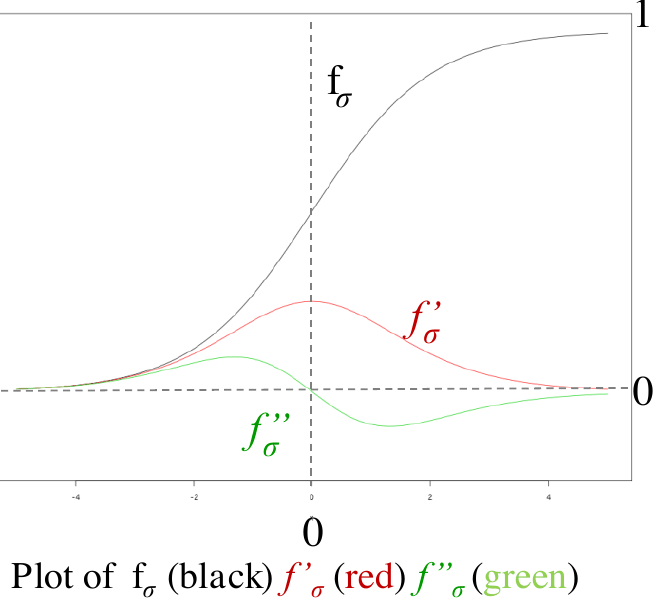
\includegraphics[width=0.43\linewidth,height=0.42\textheight,keepaspectratio]{images/06-nn1_derivate-sigmoide.png}
\caption{La logistica \(f_\sigma\) (nero), la sua derivata \(f'_\sigma\) (rosso)
e la derivata seconda \(f''_\sigma\) (verde).}
\end{figure}

È ancora una regola di \textbf{correzione dell'errore}, con alcune
osservazioni:

\begin{itemize}
\tightlist
\item
  la pendenza \(a\) influenza l'ampiezza del passo di discesa;
\item
  \(f'_\sigma\) è \textbf{massima per \(net\) vicino a 0} (zona quasi
  lineare): lì i delta possono essere grandi;
\item
  \(f'_\sigma\) è \textbf{minima nei casi saturi} (\(f\) vicino a 0 o
  1): delta piccoli, pesi che cambiano lentissimamente. Bisogna
  \textbf{evitare una saturazione prematura}, ad esempio
  \textbf{partendo con pesi piccoli}.
\end{itemize}

\begin{boxtip}{Un ponte tra LMS e Perceptron}

Quando un pattern è classificato correttamente ``con decisione'' (uscita
saturata vicino al target), \(f'_\sigma \approx 0\) e la correzione è
quasi nulla, proprio come nel Perceptron, che non corregge i pattern
corretti. Usando \(f_\sigma\) si approssima quindi non solo la LTU, ma
anche l'algoritmo del Perceptron.

\end{boxtip}

\section{Le reti neurali: il Multi-Layer
Perceptron}\label{le-reti-neurali-il-multi-layer-perceptron}

Tutti gli ingredienti sono pronti. Un \textbf{MLP} si può vedere in due
modi:

\begin{itemize}
\tightlist
\item
  \textbf{A.} come una \textbf{rete di unità interconnesse};
\item
  \textbf{B.} come una \textbf{funzione flessibile} \(h(\mathbf{x})\),
  composta da funzioni non lineari annidate.
\end{itemize}

\begin{figure}[htbp]
\centering
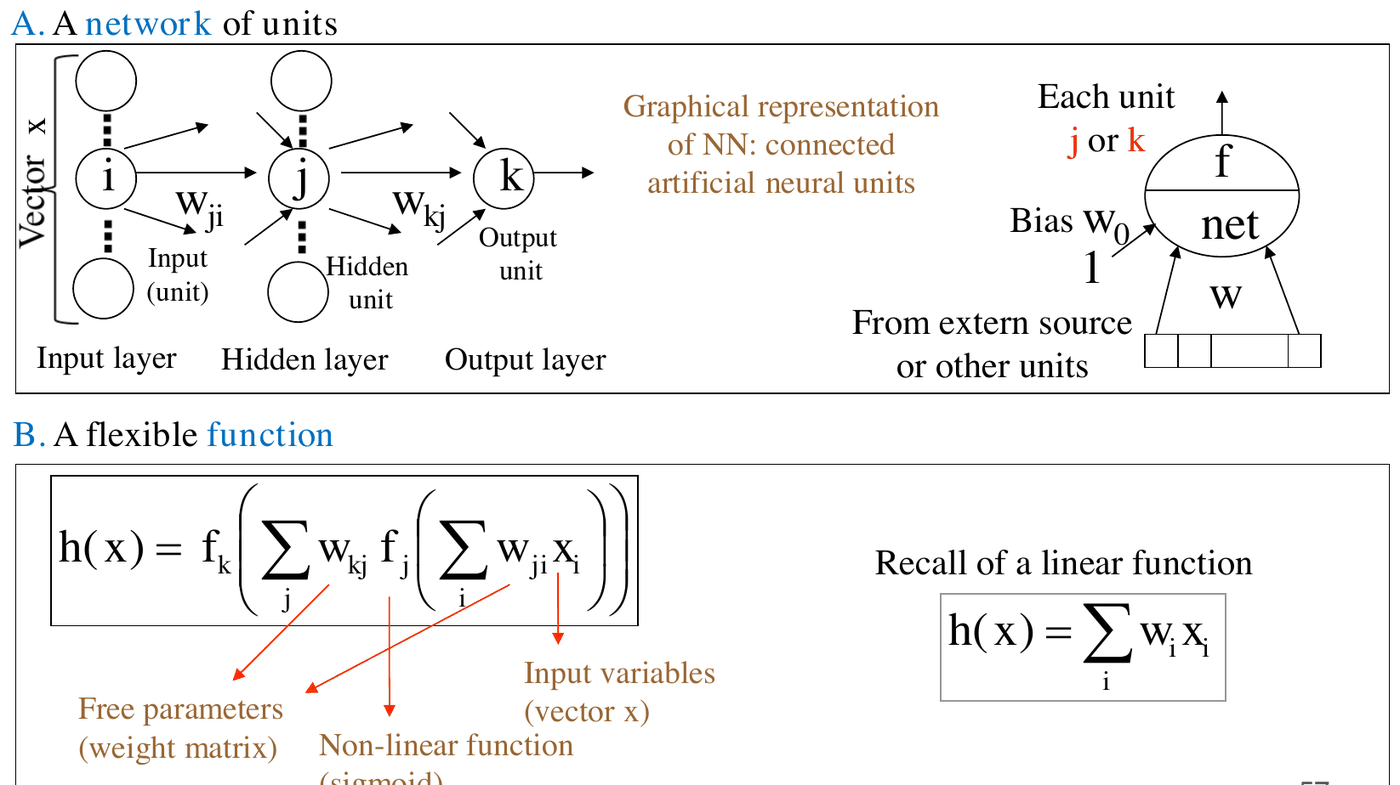
\includegraphics[width=0.91\linewidth,height=0.42\textheight,keepaspectratio]{images/06-nn1_due-viste.png}
\caption{Le due viste di una rete feedforward con uno strato nascosto: rete di
unità (A) e funzione flessibile (B).}
\end{figure}

\subsection{Vista A: una rete di
unità}\label{vista-a-una-rete-di-unituxe0}

In un'architettura MLP:

\begin{itemize}
\tightlist
\item
  le unità sono connesse da collegamenti pesati e organizzate in
  \textbf{strati} (\emph{layer});
\item
  lo \textbf{strato di input} è solo la sorgente dell'input
  \(\mathbf{x}\): carica (copia) il pattern, senza calcolare \(net\) né
  \(f\);
\item
  lo \textbf{strato nascosto} (\emph{hidden}) proietta sullo strato di
  uscita (o su un altro strato nascosto);
\item
  lo \textbf{strato di uscita} produce \(h(\mathbf{x})\).
\end{itemize}

\subsection{Vista B: una funzione
flessibile}\label{vista-b-una-funzione-flessibile}

Una rete a due strati (uno nascosto e uno di uscita) calcola \[
h(\mathbf{x}) = f_k\left(\sum_j w_{kj}\, f_j\left(\sum_i w_{ji}\, x_i\right)\right),
\] dove \(x_i\) sono le variabili di input, \(w\) i parametri liberi
(matrici dei pesi) e \(f\) funzioni non lineari (sigmoidi). Si confronti
con la funzione lineare \(h(\mathbf{x}) = \sum_i w_i x_i\): la rete è
una composizione di funzioni lineari e non lineari.

\subsection{Componenti di una rete
neurale}\label{componenti-di-una-rete-neurale}

Una rete si descrive tradizionalmente con:

\begin{itemize}
\tightlist
\item
  il tipo di \textbf{unità} (net e funzione di attivazione);
\item
  l'\textbf{architettura} (numero di unità, topologia, numero di
  strati);
\item
  l'\textbf{algoritmo di apprendimento}.
\end{itemize}

\subsection{Notazione uniforme per le
unità}\label{notazione-uniforme-per-le-unituxe0}

Per una generica unità \(t\) (che può essere nascosta, \(j\), o di
uscita, \(k\)): \[
net_t(\mathbf{x}) = \sum_u w_{tu}\, o_u, \qquad o_t(\mathbf{x}) = f_t\big(net_t(\mathbf{x})\big),
\] dove \(u\) indica una generica sorgente di input (che può essere
\(i\) o \(j\)). Caricando il pattern nello strato di input, si può usare
il simbolo \(o\) sia per gli input sia per le uscite delle unità
nascoste: l'input all'unità \(t\) dalla sorgente \(u\) (attraverso la
connessione \(w_{tu}\)) è \(o_u\). Questa notazione sarà usata nella
derivazione della backpropagation.

\begin{boxexample}{Esercizio (dalla lezione)}

\begin{enumerate}
\def\labelenumi{\arabic{enumi}.}
\tightlist
\item
  Per i pesi \(w_{ji}\) (input → nascosta), l'input \(o_u\) è
  \(o_i = x_i\), la componente del pattern.
\item
  Per i pesi \(w_{kj}\) (nascosta → uscita), l'input \(o_u\) è \(o_j\),
  l'uscita dell'unità nascosta \(j\).
\item
  \(w_{t0}\) è il \textbf{bias} di ciascuna unità \(t\), con input
  costante \(o_0 = 1\).
\item
  Unità nascosta: \(o_j = f_j\left(\sum_i w_{ji}\,x_i\right)\); unità di
  uscita: \(o_k = f_k\left(\sum_j w_{kj}\,o_j\right)\).
\end{enumerate}

\end{boxexample}

\subsection{Architettura e processing
feedforward}\label{architettura-e-processing-feedforward}

L'\textbf{architettura} definisce la topologia delle connessioni. La
rete a due strati descritta sopra è l'MLP standard,
\textbf{completamente connesso}; si possono avere più strati nascosti e
anche connessioni che ``saltano'' strati.

\begin{figure}[htbp]
\centering
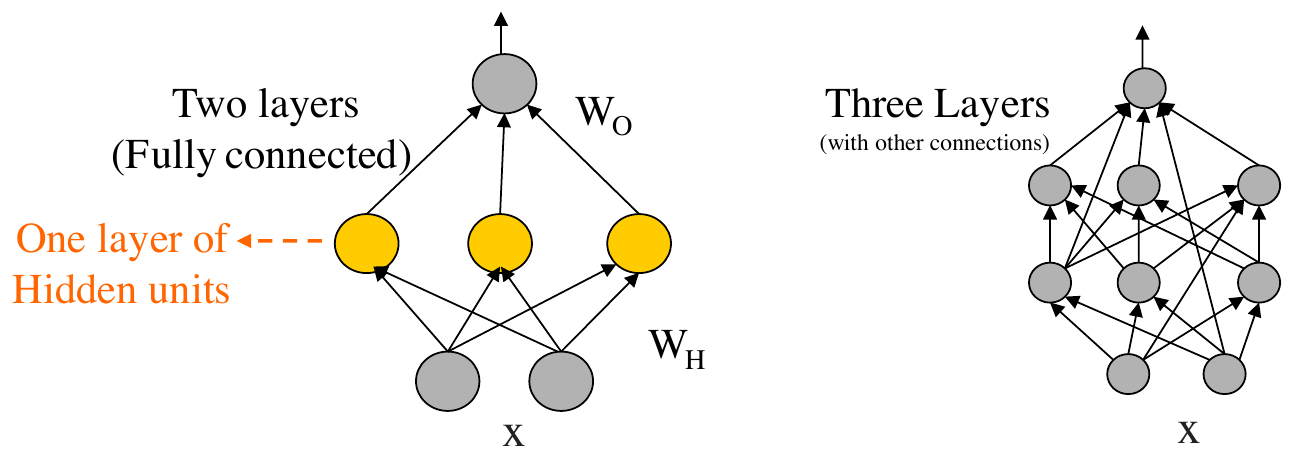
\includegraphics[width=0.71\linewidth,height=0.42\textheight,keepaspectratio]{images/06-nn1_architettura.png}
\caption{Architetture MLP: due strati completamente connessi (sinistra), tre
strati con altre connessioni (destra).}
\end{figure}

L'elaborazione \textbf{feedforward} di un pattern procede dall'input
all'uscita:

\begin{enumerate}
\def\labelenumi{\arabic{enumi}.}
\tightlist
\item
  si carica il pattern \(\mathbf{x}\) nello strato di input;
\item
  si calcolano le uscite di tutte le unità del primo strato nascosto;
\item
  poi del secondo strato nascosto, e così via;
\item
  si calcolano le uscite dello strato di uscita, cioè \(h(\mathbf{x})\);
\item
  si può ora calcolare l'errore (delta) in uscita.
\end{enumerate}

\begin{boxnote}{Reti ricorrenti}

Le reti \textbf{feedforward} hanno un'unica direzione input → output. Le
\textbf{reti ricorrenti} aggiungono connessioni di feedback (cicli): i
self-loop danno alla rete proprietà dinamiche e una \textbf{memoria}
delle computazioni passate, estendendo il modello all'elaborazione di
\textbf{sequenze} (e dati strutturati). Saranno trattate in una lezione
dedicata.

\end{boxnote}

\section{Perché le reti neurali sono
flessibili}\label{perchuxe9-le-reti-neurali-sono-flessibili}

Tre domande guidano l'analisi: perché le reti sono un modello flessibile
(e si possono vedere come LBE)? La flessibilità è teoricamente fondata?
Come si apprendono i pesi?

\subsection{Quali task}\label{quali-task}

Lo spazio delle ipotesi è lo \textbf{spazio continuo di tutte le
funzioni} rappresentabili assegnando valori ai pesi di un'architettura
data. A seconda delle unità di uscita, la rete tratta:

\begin{itemize}
\tightlist
\item
  \textbf{classificazione}, con uscita sigmoidale;
\item
  \textbf{regressione}, con uscita lineare.
\end{itemize}

Con \textbf{più unità di uscita} si ottengono regressione multipla o
classificatori multi-classe (ad esempio tre uscite che danno
\(0{,}2;\ 0{,}7;\ 0{,}1\) per tre classi).

\begin{figure}[htbp]
\centering
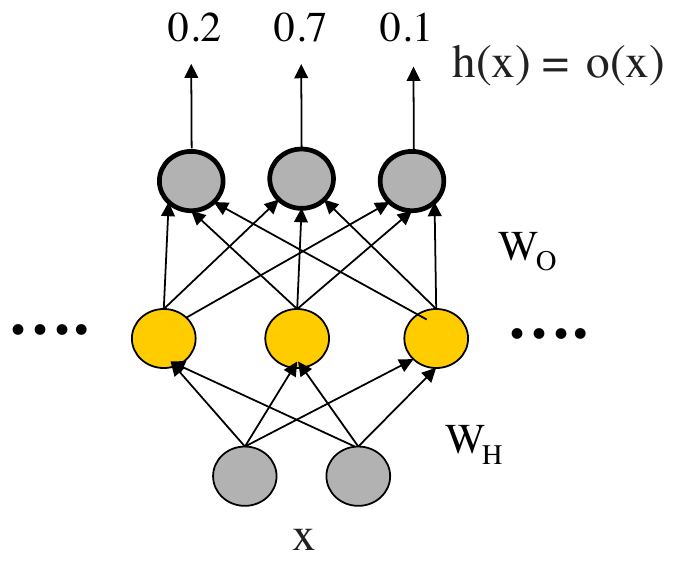
\includegraphics[width=0.37\linewidth,height=0.42\textheight,keepaspectratio]{images/06-nn1_multi-output.png}
\caption{Una rete con uscite multiple per un problema multi-classe.}
\end{figure}

\subsection{La rete come espansione in basi
adattiva}\label{la-rete-come-espansione-in-basi-adattiva}

La rete calcola
\(h(\mathbf{x}) = f_k\left(\sum_j w_{kj}\,f_j\left(\sum_i w_{ji}x_i\right)\right)\).
Unità e architettura sono solo una rappresentazione grafica del flusso
dei dati. Ogni termine \[
\phi_j(\mathbf{x}, \mathbf{w}) = f_j\left(\sum_i w_{ji}\,x_i\right)
\] può essere visto come calcolato da un'unità nascosta indipendente,
oppure come una \textbf{funzione di base \(\phi\) di una LBE}.
Confrontiamo:

\begin{itemize}
\tightlist
\item
  \textbf{LBE}: \(h(\mathbf{x}) = \sum_j w_j\,\phi_j(\mathbf{x})\)
  (regressione) o
  \(h(\mathbf{x}) = f\left(\sum_j w_j\,\phi_j(\mathbf{x})\right)\)
  (classificazione), con le \(\phi\) \textbf{fissate a priori} e il
  modello lineare nei parametri.
\item
  \textbf{Rete neurale}:
  \(h(\mathbf{x}) = f_k\left(\sum_j w_{kj}\,\phi_j(\mathbf{x}, \mathbf{w})\right)\),
  dove ora \textbf{le \(\phi\) dipendono dai pesi} e quindi \textbf{si
  adattano ai dati} durante l'addestramento.
\end{itemize}

\begin{boxtip}{Le reti neurali come basi adattive}

Le reti neurali sono un approccio a \textbf{funzioni di base adattive}:
le basi stesse vengono adattate ai dati (apprendendo i \(\mathbf{w}\)
dentro le \(\phi\)). Tutte le basi hanno lo stesso tipo (dato dalla
funzione di attivazione). \(h(\mathbf{x})\) è una funzione non lineare
di somme pesate di modelli lineari trasformati in modo non lineare, con
il miglioramento cruciale dell'\textbf{adattività}. (Da confrontare più
avanti con le SVM, un'altra forma di LBE.)

\end{boxtip}

Ogni unità nascosta calcola una nuova \textbf{feature derivata non
lineare}, in modo adattivo. In altre parole: la capacità rappresentativa
del modello è legata alla presenza di uno \textbf{strato nascosto con
attivazioni non lineari}, che trasforma l'input nella
\textbf{rappresentazione interna} della rete. L'apprendimento definisce
una rappresentazione interna adatta, cioè nuove feature nascoste dei
dati, che permettono al modello di estrarre le \textbf{statistiche di
ordine superiore} rilevanti per approssimare la funzione target.

\begin{boxwarning}{Le unità nascoste devono essere non lineari}

Un MLP con unità \textbf{lineari} equivale a una rete a \textbf{un solo
strato}: la composizione di funzioni lineari è lineare. Con \(f\)
identità,
\(h(\mathbf{x}) = \sum_j w_{kj}\sum_i w_{ji}x_i = \sum_i\left(\sum_j w_{kj}w_{ji}\right)x_i = \sum_i w'_i x_i\).

Il prezzo della non linearità: il modello è \textbf{non lineare nei
parametri} \(\mathbf{w}\), e l'addestramento diventa un problema di
\textbf{ottimizzazione non lineare} (non convesso).

\end{boxwarning}

\subsection{L'approssimazione
universale}\label{lapprossimazione-universale}

\begin{boxtheorem}{Teorema di approssimazione universale (Cybenko 1989, Hornik et al.)}

Una rete con \textbf{un solo strato nascosto} (con attivazioni
logistiche) e uscita lineare può approssimare arbitrariamente bene
\textbf{ogni funzione continua} (su ipercubi), purché ci siano
abbastanza unità nascoste: dati \(f\) ed \(\varepsilon > 0\), esiste
\(h\) tale che \(|f(\mathbf{x}) - h(\mathbf{x})| < \varepsilon\) per
ogni \(\mathbf{x}\) nell'ipercubo. Più in generale, un MLP può
approssimare arbitrariamente bene ogni mappatura input-output, con
abbastanza unità nascoste.

\end{boxtheorem}

(Si può pensare a una generalizzazione dell'approssimazione con serie di
Fourier finite.)

\begin{boxwarning}{È un teorema di esistenza}

Il teorema dice che la rete \textbf{esiste}, ma non fornisce né
l'\textbf{algoritmo} per trovarla né il \textbf{numero di unità}
necessario.

\end{boxwarning}

Restano quindi due questioni fondamentali: \textbf{come apprendere} (la
backpropagation, prossima lezione) e \textbf{come scegliere
l'architettura}.

\subsection{Potere espressivo e
VC-dimension}\label{potere-espressivo-e-vc-dimension}

Il potere espressivo di una rete dipende dal \textbf{numero di unità} e
dalla loro \textbf{configurazione}. Il numero di unità è legato alla
VC-dimension: le capacità della rete dipendono dal numero di parametri
(in un MLP completamente connesso, circa il numero di input per il
numero di unità nascoste, più le unità nascoste per le uscite), ma anche
dal \textbf{valore} dei pesi:

\begin{itemize}
\tightlist
\item
  pesi \(= 0\) → VC-dim minima;
\item
  pesi piccoli → si lavora nella parte lineare della sigmoide → VC-dim
  piccola;
\item
  pesi grandi → modello più complesso.
\end{itemize}

Poiché l'addestramento parte da pesi vicini a 0 e i pesi crescono
durante il training, la rete è uno \textbf{spazio delle ipotesi di
dimensione variabile}: la VC-dim effettiva cresce durante
l'apprendimento. (Questo sarà la base dell'\emph{early stopping}.)

\subsection{Quanti strati?
(anticipazione)}\label{quanti-strati-anticipazione}

Il teorema di approssimazione universale dice che uno strato nascosto
basta, ma non garantisce che basti un numero \textbf{piccolo} di unità.
Esistono risultati di tipo ``\emph{no flattening}'' (sull'efficienza,
non sull'espressività): funzioni che con un solo strato nascosto
richiederebbero un numero \textbf{esponenziale} di unità (rispetto alla
dimensione dell'input), mentre con più strati ne bastano molte meno. Ma
è facile addestrare un MLP con molti strati? Lo vedremo nel deep
learning.

\subsection{Il bias induttivo delle reti
neurali}\label{il-bias-induttivo-delle-reti-neurali}

Per le reti addestrate con backpropagation, il bias induttivo è legato
alle proprietà di \textbf{smoothness} delle funzioni: piccole variazioni
dell'input producono piccole variazioni dell'output (ad esempio,
derivata prima localmente limitata). È un'assunzione molto comune nel
ML, ed è ragionevole: se la funzione target non è liscia (ad esempio un
generatore di numeri casuali), la generalizzazione è comunque
impossibile.

\section{Verso l'algoritmo di
apprendimento}\label{verso-lalgoritmo-di-apprendimento}

L'algoritmo di apprendimento adatta i pesi della rete per ottenere la
migliore approssimazione della funzione target, minimizzando come sempre
una funzione d'errore (o loss) sui dati di training.

\subsection{Il problema del credit
assignment}\label{il-problema-del-credit-assignment}

\begin{itemize}
\tightlist
\item
  Il Perceptron ha un algoritmo di apprendimento, ma non rappresenta
  tutte le funzioni booleane.
\item
  Una rete di perceptron rappresenta ogni funzione booleana, ma serve un
  algoritmo per addestrarla.
\end{itemize}

Cosa cambia? Il \textbf{problema del credit assignment}: quanta
``responsabilità'' dell'errore attribuire alle unità nascoste? Per le
unità di uscita conosciamo la risposta desiderata e quindi l'errore; per
le unità nascoste \textbf{non sappiamo quale dovrebbe essere la loro
uscita}, quindi il segnale d'errore non è direttamente misurabile. In
più, il modello è non lineare nei pesi.

Minsky e Papert (1969) ritenevano il problema troppo difficile; fu
risolto da diversi ricercatori con l'algoritmo di
\textbf{backpropagation}, reso popolare da Rumelhart, Hinton e Williams
nel libro \emph{PDP} (1986): fu il \textbf{rinascimento} delle reti
neurali.

\subsection{Il loading problem}\label{il-loading-problem}

\begin{boxdefinition}{Loading problem}

Data una rete e un insieme di esempi, esiste un insieme di pesi per cui
la rete è consistente con gli esempi? (``Caricare'' i dati di training
nei parametri liberi della rete.)

\end{boxdefinition}

Il loading problem è \textbf{NP-completo} (Judd, 1990): non è noto un
algoritmo polinomiale. In pratica, però, le reti si addestrano in tempi
ragionevoli con la backpropagation, anche se la soluzione ottima non è
garantita.

\subsection{L'idea chiave: estendere la discesa del
gradiente}\label{lidea-chiave-estendere-la-discesa-del-gradiente}

La discesa del gradiente che minimizza una loss \textbf{si estende agli
MLP}, purché loss e funzioni di attivazione siano
\textbf{differenziabili}: si tratta di trovare il delta per
\textbf{ogni} unità della rete. Il problema resta lo stesso: dati \(l\)
esempi \((\mathbf{x}_p, d_p)\) e una loss \(L\) (ad esempio
\(L(h(\mathbf{x}_p), d_p) = (d_p - h_\mathbf{w}(\mathbf{x}_p))^2\)),
trovare \(\mathbf{w}\) che minimizzi \[
E(\mathbf{w}) = R_{emp} = \frac{1}{l}\sum_{p=1}^{l}\big(d_p - h(\mathbf{x}_p)\big)^2
\] calcolandone il gradiente. Servono: loss differenziabile, attivazioni
differenziabili e una rete per seguire il flusso dell'informazione.

Proprietà della backpropagation:

\begin{itemize}
\tightlist
\item
  è semplice grazie alla \textbf{forma composizionale} del modello;
\item
  usa solo quantità \textbf{locali} a ogni unità, preservandone la
  modularità;
\item
  è \textbf{efficiente}: \(O(\#W)\) invece di \(O(\#W^2)\), grazie alla
  fattorizzazione dei delta;
\item
  sulla plausibilità biologica il dibattito è aperto (si è ipotizzato
  che il cervello usi un'approssimazione locale subottima della BP).
\end{itemize}

La derivazione completa è nella prossima lezione (e nelle note
\href{07\%20-\%20Note\%20sulla\%20backpropagation}{07 - Note sulla
backpropagation}).

\subsection{Questioni pratiche
nell'addestramento}\label{questioni-pratiche-nelladdestramento}

Il modello è spesso \textbf{sovra-parametrizzato} e l'ottimizzazione è
\textbf{non convessa} e potenzialmente instabile. Le questioni da
affrontare (dopo la backpropagation) sono: valori iniziali dei pesi,
learning rate, on-line/batch; overfitting e regolarizzazione; scalatura
dell'input e rappresentazione dell'output; numero di unità nascoste;
minimi multipli; criteri di arresto.

\begin{boxabstract}{Sintesi}

Il neurone artificiale calcola \(o = f(\sum_j w_j x_j)\). Il
\textbf{Perceptron} (soglia) ha un algoritmo di apprendimento che
\textbf{converge in un numero finito di passi} per problemi linearmente
separabili, ma non rappresenta lo XOR. Reti di perceptron a due strati
rappresentano ogni funzione booleana grazie alla
\textbf{ri-rappresentazione interna} dello strato nascosto. Sostituendo
la soglia con una \textbf{sigmoide} differenziabile si può usare la
discesa del gradiente. L'\textbf{MLP} è una funzione annidata
\(h(\mathbf{x}) = f_k(\sum_j w_{kj} f_j(\sum_i w_{ji} x_i))\),
interpretabile come \textbf{espansione in basi adattiva}, ed è un
\textbf{approssimatore universale}. Per addestrarlo bisogna risolvere il
\textbf{credit assignment} delle unità nascoste: lo fa la
backpropagation.

\end{boxabstract}

\begin{boxquestion}{Possibili domande d'esame}

\begin{itemize}
\tightlist
\item
  Descrivere il neurone artificiale e le principali funzioni di
  attivazione.
\item
  Come si rappresentano AND, OR, NOT con un perceptron? Come si risolve
  lo XOR?
\item
  Scrivere l'algoritmo di apprendimento del Perceptron.
\item
  Enunciare e dimostrare il teorema di convergenza del Perceptron.
\item
  Differenze tra algoritmo del Perceptron e LMS; perché l'LMS può
  sbagliare su problemi separabili?
\item
  Derivare la regola di aggiornamento per una singola unità sigmoidale.
\item
  Perché le unità nascoste devono essere non lineari?
\item
  In che senso una rete neurale è una LBE adattiva?
\item
  Enunciare il teorema di approssimazione universale e discuterne i
  limiti.
\item
  Cos'è il problema del credit assignment? E il loading problem?
\end{itemize}

\end{boxquestion}
